\chapter{Výsledky}
Zkoumali jsme molekuly $\mathrm{BeH/BeH^-}$ a $\mathrm{OH/OH^-}$, protože se jedná o 
molekuly, které mají vázaný jak základní stav, tak anion, a zároveň se jedná o 
dostatečně malé systémy, aby bylo možné provádět výpočty přesnými metodami.

Ke kvantově chemickým výpočtům jsme používali program MOLPRO.\cite{MOLPRO-WIREs}\cite{MOLPRO}. 
Pro určitý soubor mezijaderných vzdáleností\footnote{cca 35 hodnot} jsme napočítali 
energii základního stavu molekuly pro fixovaná jádra, u základního stavu, tak u 
aniontu. Ze znalosti těchto křivek jsme poté zjišťovali parametry molekul, které je 
možné nalézt experimentálně, což jsou disociační energie aniontu i neutrální molekuly a 
elektronové afinity vázané i úplně disociované\footnote{Ta odpovídá odpovídá 
elektronové afinitě některého z prvků v molekule.} molekuly. Protože ale experimentální 
data nejsou určená minimem potenciální energie molekuly, ale základní vibrační 
hladinou, bylo třeba napočítat energetické hladiny získaného potenciálu. K tomu jsme 
použili \? metodu výpočtu na na mříži \? . Vzhledem k počtu geometrií, pro které jsme 
prováděli kvantově-chemické výpočty, který byl nedostatečný pro další numerické výpočty
\footnote{a extrémní výpočetní náročnosti při případném výpočtu v dostatečném počtu 
geometrií}, jsme získané hodnoty proložili kubickým splinem, ze kterého jsme pak 
interpolovali hodnotu potenciálu v několika stovkách bodů. Poté jsme numericky získali 
energetické hladiny v daném potenciálové křivce pro částici o (redukované) hmotnosti $
\mu = m_1m_2/(m_1+m_2)$, kde $m_1,m_2$ jsou hmotnosti jednotlivých jader. Získané 
vlastní stavy pak odpovídají vibračním stavům dané molekuly.

\begin{figure}
\centering
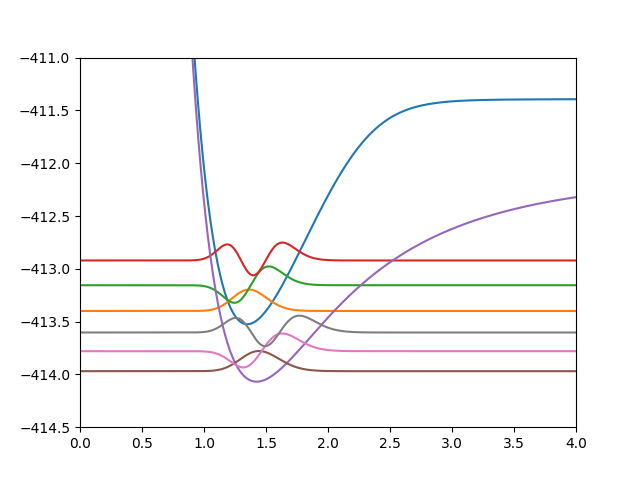
\includegraphics[width=0.8\textwidth]{../img/VibrStavy1.png}
\caption{Nejnižší vibrační hladiny molekul $\mathrm{BeH/BeH^-}$}
\label{Vibr1}
\end{figure}
\ltable{../tbl/BeH.tex}{BeH}
\ltable{../tbl/OH.tex}{OH}

\begin{tabular}{rrrrr}
\toprule
Method & $v_0 [\mathrm{eV}]$ & $v_1 [\mathrm{eV}]$ & $v_2 [\mathrm{eV}]$ & $v_3[\mathrm{eV}]$ \\ \midrule
    FCI  /aug-cc-pVDZ & 0.1240 & 0.3648 & 0.5953 & 0.8152\\
RCCSD(T)  /aug-cc-pVDZ & 0.1244 & 0.3661 & 0.5975 & 0.8186\\
CI 5,1,1,0 /aug-cc-pVDZ & 0.1240 & 0.3649 & 0.5954 & 0.8153\\
CI 6,2,2,0 /aug-cc-pVDZ & 0.1240 & 0.3648 & 0.5953 & 0.8152\\
FCI  /aug-cc-pCVDZ & 0.1245 & 0.3658 & 0.5966 & 0.8168\\
RCCSD(T)  /aug-cc-pCVDZ & 0.1249 & 0.3670 & 0.5988 & 0.8201\\
CI 5,1,1,0 /aug-cc-pCVDZ & 0.1245 & 0.3658 & 0.5967 & 0.8169\\
CI 6,2,2,0 /aug-cc-pCVDZ & 0.1245 & 0.3658 & 0.5966 & 0.8168\\
FCI  /cc-pVTZ & 0.1254 & 0.3688 & 0.6021 & 0.8252\\
RCCSD(T)  /cc-pVTZ & 0.1257 & 0.3698 & 0.6039 & 0.8281\\
CI 6,2,2,0 /cc-pVTZ & 0.1254 & 0.3688 & 0.6021 & 0.8252\\
FCI  /aug-cc-pVTZ & 0.1252 & 0.3682 & 0.6010 & 0.8234\\
RCCSD(T)  /aug-cc-pVTZ & 0.1255 & 0.3692 & 0.6028 & 0.8263\\
CI 6,2,2,0 /aug-cc-pVTZ & 0.1254 & 0.3691 & 0.6032 & 0.8275\\
RCCSD(T)  /aug-cc-pVQZ & 0.1261 & 0.3713 & 0.6065 & 0.8314\\
CI 5,1,1,0 /aug-cc-pVQZ & 0.1258 & 0.3704 & 0.6047 & 0.8287\\
CI 6,2,2,0 /aug-cc-pVQZ & 0.1258 & 0.3704 & 0.6047 & 0.8286\\
CI 9,3,3,1 /aug-cc-pVQZ & 0.1258 & 0.3704 & 0.6047 & 0.8286\\
CI 5,1,1,0 /aug-cc-pV5Z & 0.1259 & 0.3707 & 0.6052 & 0.8293\\
CI 6,2,2,0 /aug-cc-pV5Z & 0.1259 & 0.3707 & 0.6052 & 0.8293\\
\bottomrule
\end{tabular}
    
\begin{table}[]
\centering
\caption{OH vibration states}
\label{TODO}
\begin{tabular}{rrrrr}
\toprule
Method & $v_0 [" eV"]$ & $v_1 [" eV"]$ & $v_2 [" eV"]$ & $v_3[" eV"]$ \\ \midrule
CI 4,1,1,0 /aug-cc-pVDZ & 0.225 & 0.657 & 1.065 & 1.451\\
CI 4,2,2,0 /aug-cc-pVDZ & 0.224 & 0.656 & 1.063 & 1.448\\
CI 6,2,2,0 /aug-cc-pVDZ & 0.224 & 0.656 & 1.064 & 1.450\\
CI 8,2,2,0 /aug-cc-pVDZ & 0.224 & 0.656 & 1.063 & 1.449\\
CI 4,1,1,0 /aug-cc-pVTZ & 0.227 & 0.665 & 1.081 & 1.474\\
CI 4,2,2,0 /aug-cc-pVTZ & 0.227 & 0.664 & 1.078 & 1.469\\
CI 6,2,2,0 /aug-cc-pVTZ & 0.227 & 0.664 & 1.079 & 1.473\\
CI 8,2,2,0 /aug-cc-pVTZ & 0.227 & 0.664 & 1.078 & 1.471\\
CI 4,1,1,0 /aug-cc-pVQZ & 0.228 & 0.668 & 1.085 & 1.481\\
CI 4,2,2,0 /aug-cc-pVQZ & 0.227 & 0.665 & 1.080 & 1.474\\
CI 6,2,2,0 /aug-cc-pVQZ & 0.227 & 0.667 & 1.084 & 1.479\\
CI 8,2,2,0 /aug-cc-pVQZ & 0.227 & 0.666 & 1.083 & 1.477\\
\bottomrule
\end{tabular}
\end{table}
    
\begin{tabular}{rrrrr}
\toprule
Method & $v_0 [\mathrm{eV}]$ & $v_1 [\mathrm{eV}]$ & $v_2 [\mathrm{eV}]$ & $v_3[\mathrm{eV}]$ \\ \midrule
CI 4,1,1,0 /aug-cc-pVDZ & 0.228 & 0.662 & 1.069 & 1.449\\
CI 4,2,2,0 /aug-cc-pVDZ & 0.221 & 0.647 & 1.047 & 1.426\\
CI 6,2,2,0 /aug-cc-pVDZ & 0.224 & 0.655 & 1.059 & 1.440\\
CI 8,2,2,0 /aug-cc-pVDZ & 0.224 & 0.653 & 1.057 & 1.437\\
CI 4,1,1,0 /aug-cc-pVTZ & 0.212 & 0.637 & 1.047 & 1.448\\
CI 4,2,2,0 /aug-cc-pVTZ & 0.221 & 0.649 & 1.054 & 1.439\\
CI 6,2,2,0 /aug-cc-pVTZ & 0.225 & 0.661 & 1.072 & 1.460\\
CI 8,2,2,0 /aug-cc-pVTZ & 0.225 & 0.660 & 1.070 & 1.457\\
CI 4,1,1,0 /aug-cc-pVQZ & 0.212 & 0.637 & 1.052 & 1.455\\
CI 4,2,2,0 /aug-cc-pVQZ & 0.224 & 0.657 & 1.066 & 1.450\\
CI 6,2,2,0 /aug-cc-pVQZ & 0.225 & 0.663 & 1.077 & 1.467\\
CI 8,2,2,0 /aug-cc-pVQZ & 0.225 & 0.662 & 1.075 & 1.463\\
\bottomrule
\end{tabular}
    